% vim:ts=4:sw=4
%
% Copyright (c) 2008-2009 solvethis
% Copyright (c) 2010-2015 Casper Ti. Vector
% Public domain.
%
% 使用前请先仔细阅读 pkuthss 和 biblatex-caspervector 的文档,
% 特别是其中的 FAQ 部分和用红色强调的部分。
% 两者可在终端/命令提示符中用
%   texdoc pkuthss
%   texdoc biblatex-caspervector
% 调出。

% 采用了自定义的(包括大小写不同于原文件的)字体文件名,
% 并改动 ctex.cfg 等配置文件的用户请自行加入 nofonts 选项;
% 其它用户不用加入 nofonts 选项,加入之后反而会产生错误。
%
% 图书馆要求电子版论文的目录必须为黑色,
% 且某些教务要求打印版论文的文字部分为纯黑色而非灰度打印,
% 【因此最终打印和提交论文前,请将“colorlinks”改为“nocolorlinks”。】
\documentclass[UTF8, colorlinks]{pkuthss}

% 使用 biblatex 排版参考文献,并规定其格式。
%
% 如果无法使用 biber,可以把“backend = biber”改为“backend = bibtex”,
% 并改用 bibtex 产生参考文献,详见 pkuthss 的文档。
% 使用 biber 时,请去掉所有的 sorting 选项,否则会出错。
%
% 默认按照引用顺序排序(“sorting = none”),详见 biblatex-caspervector 的文档
% (因为是默认设置所以其实不用写,不过出于完备性的考虑仍然在这里列出)。
% 若需要按照英文文献在前,中文文献在后排序,请设置“sorting = ecnty”;
% 若需要按照中文文献在前,英文文献在后排序,请设置“sorting = centy”。
\usepackage[backend = biber, style = caspervector, utf8, sorting = none]{biblatex}
% 提供近似于学校所要求的 Times New Roman / Arial 的字体。
\usepackage[defaultsups]{newtxtext}
\usepackage{newtxmath}
% 产生 originauth.tex 里的 \square。
\usepackage{amssymb}
\usepackage{float}
\usepackage{subfig}
\usepackage{amsmath}
\usepackage{amssymb}
\DeclareMathOperator*{\argmax}{argmax}

% 按学校要求设定参考文献列表中的条目之内及之间的距离。
\setlength{\bibitemsep}{3bp}
% 对于 linespread 值的计算过程有兴趣的同学可以参考 pkuthss-extra.sty。
\setcounter{secnumdepth}{3}
%设置subsubsection序号
\renewcommand*{\bibfont}{\zihao{5}\linespread{1.27}\selectfont}

% 设定文档的基本信息。
\pkuthssinfo{
	cthesisname = {本科生毕业论文}, ethesisname = {Undergraduate Thesis},
	ctitle = {基于人脸识别的轻量级社交平台}, etitle = {Test Document},
	cauthor = {佘俊峰},
	eauthor = {Test},
	studentid = {1100012769},
	date = {二〇一五年五月},
	school = {信息科学技术学院},
	cmajor = {计算机}, emajor = {Some Major},
	direction = {移动互联网},
	cmentor = {边凯归}, ementor = {Prof.\ Somebody},
	ckeywords = {人脸识别,图片社交应用,移动设备,匹配算法}, ekeywords = {First, Second}
}
% 载入参考文献数据库(注意不要省略“.bib”)。
\addbibresource{thesis.bib}
% \CTEXsetup[name={第~,~小节}]{subsubsection}
% 普通用户可删除此段。
\usepackage{color}
\def\pkuthssffaq{%
	\emph{\textcolor{red}{pkuthss 文档模版最常见问题:}}

	在最终打印和提交论文之前,
	请将 pkuthss 文档类选项中的 %
	\texttt{colorlinks} 改为 \texttt{nocolorlinks},
	因为图书馆要求电子版论文的目录必须为黑色,
	且某些教务要求打印版论文的文字部分为纯黑色而非灰度打印。

	\texttt{\string\cite}、\texttt{\string\parencite} %
	和 \texttt{\string\supercite} 三个命令分别产生%
	未格式化的、带方括号的和上标且带方括号的引用标记:%
	\cite{test-en},\parencite{test-zh}、\supercite{test-en, test-zh}。

	若要避免章末空白页,请在调用 pkuthss 文档类时加入 \texttt{openany} 选项。

	如果编译时不出参考文献,
	请参考 \texttt{texdoc pkuthss}“问题及其解决”一章
	“其它可能存在的问题”一节中关于 biber 的说明。
}

\begin{document}
	% 以下为正文之前的部分,默认不进行章节编号。
	\frontmatter
	% 此后到下一 \pagestyle 命令之前不排版页眉或页脚。
	\pagestyle{empty}

	% 自动生成标题页。
	\maketitle
	% 版权声明。
	% vim:ts=4:sw=4
%
% Copyright (c) 2008-2009 solvethis
% Copyright (c) 2010-2015 Casper Ti. Vector
% All rights reserved.
%
% Redistribution and use in source and binary forms, with or without
% modification, are permitted provided that the following conditions are
% met:
%
% * Redistributions of source code must retain the above copyright notice,
%   this list of conditions and the following disclaimer.
% * Redistributions in binary form must reproduce the above copyright
%   notice, this list of conditions and the following disclaimer in the
%   documentation and/or other materials provided with the distribution.
% * Neither the name of Peking University nor the names of its contributors
%   may be used to endorse or promote products derived from this software
%   without specific prior written permission.
%
% THIS SOFTWARE IS PROVIDED BY THE COPYRIGHT HOLDERS AND CONTRIBUTORS "AS
% IS" AND ANY EXPRESS OR IMPLIED WARRANTIES, INCLUDING, BUT NOT LIMITED TO,
% THE IMPLIED WARRANTIES OF MERCHANTABILITY AND FITNESS FOR A PARTICULAR
% PURPOSE ARE DISCLAIMED. IN NO EVENT SHALL THE COPYRIGHT HOLDER OR
% CONTRIBUTORS BE LIABLE FOR ANY DIRECT, INDIRECT, INCIDENTAL, SPECIAL,
% EXEMPLARY, OR CONSEQUENTIAL DAMAGES (INCLUDING, BUT NOT LIMITED TO,
% PROCUREMENT OF SUBSTITUTE GOODS OR SERVICES; LOSS OF USE, DATA, OR
% PROFITS; OR BUSINESS INTERRUPTION) HOWEVER CAUSED AND ON ANY THEORY OF
% LIABILITY, WHETHER IN CONTRACT, STRICT LIABILITY, OR TORT (INCLUDING
% NEGLIGENCE OR OTHERWISE) ARISING IN ANY WAY OUT OF THE USE OF THIS
% SOFTWARE, EVEN IF ADVISED OF THE POSSIBILITY OF SUCH DAMAGE.

\chapter*{版权声明}
\thispagestyle{empty}

任何收存和保管本论文各种版本的单位和个人,
未经本论文作者同意,不得将本论文转借他人,
亦不得随意复制、抄录、拍照或以任何方式传播。
否则一旦引起有碍作者著作权之问题,将可能承担法律责任。

% 若需排版二维码,请将二维码图片重命名为“barcode”,
% 转为合适的图片格式,并放在当前目录下,然后去掉下面 3 行的注释。
%\vfill\noindent
%\includegraphics[height = 5em]{barcode}



	% 此后到下一 \pagestyle 命令之前正常排版页眉和页脚。
	% \cleardoublepage
	\pagestyle{plain}
	% 重置页码计数器,用大写罗马数字排版此部分页码。
	\setcounter{page}{0}
	\pagenumbering{Roman}

	% 中英文摘要。
	% vim:ts=4:sw=4
% Copyright (c) 2014 Casper Ti. Vector
% Public domain.

\begin{cabstract}
	% 中文测试文字。
	% \pkuthssffaq
	人际关系总是人们生活中非常重要的一环,⼈们扩展自己的交际圈的需求⽆所不在,在如今的互联网的时代下,移动应用成为了人们进行社交活动的重要方式。为了尽可能减少用户去扩展社交圈的障碍,令⽤户可以更加有效地获取新的人际关系,很多的移动互联⽹应用尝试用不同的方式去 降低用户获取好友的难度。然⽽,这些现有的应用对于用户的信息利用不完全,往往不能提供令用户满意的效果。

	本⽂提出了⼀种通过人脸识别的技术为主,用户的的其他信息为辅助的方法来帮助用户去减少他们去扩展社交圈的难度,在本系统中,将用户的人脸看做了一个非常重要的特征,来配合其他特征来进行匹配算法,为用户推荐好友。 

针对以上的想法,本⽂实现了一种适合多移动平台,覆盖广泛的应用,并设计了不同的匹配算法,通过实验衡量其性能和用户体验。最终确定了一个比较优秀的设计 成为了一个移动互联⽹应⽤,经实验证明该应用具有良好的体验,可以面向商⽤进⼀步推⼴。
而更进一步的,由于图片流应用的火热和现在computer version技术的发展,可以根据人们在日常生活中所表现出的倾向进行学习和进一步的匹配,前景十分远大。


\end{cabstract}

\begin{eabstract}
	Personal relationship is always most important part in human's live, thus people are inclined to expand their relatioship. In the internet age, mobile application become the most popular access to communicate with others. To facilitate people developing relationship, there are a myriad ways supporing by current application to find friends. 
	However, lack of taking advantage of full of user information, the ways to find friends could not lead to a good result.

	Therefore, regarding this problem, we introduce face recognition to facilitate user extending their social circle. Recommend friends to user mainly by the features of user's face, associating with other user information. Further we devise several matching friend algorthm, implement a application suited multiple mobile platform to realize it. And the user study shows that the social application based on face recogition has a good performance to extend user social circle. 

	Moreover, this matching algorithm could achieve more higher by the development of computer version technologies.   
\end{eabstract}


	% 自动生成目录。
	\tableofcontents

	% 以下为正文部分,默认要进行章节编号。
	\mainmatter
	% 序言。
	% vim:ts=4:sw=4
% Copyright (c) 2014 Casper Ti. Vector
% Public domain.

\specialchap{序言}
% 中文测试文字。
\pkuthssffaq


	% 各章节。
	% vim:ts=4:sw=4
% Copyright (c) 2014 Casper Ti. Vector
% Public domain.

\chapter{引言}
\section{背景分析}
随着网络和移动设备普及,人们越来越多的用移动设备来进行自己的社交活动,现在层出不穷的社交类应用一种在涌现,更为显著的是wechat其生态圈已经成为了中国用户一种特定的生活模式,所以移动应用在人们社交关系中起到的作用不言而喻。

并且在这个信息爆炸时代下,由于大量的信息涌到人们眼前,而不断兴起的社交媒体更是进一步将信息碎片化。不像文字一般,照片、图像作为不易切割的单位在传递信息过程中备受用户青睐。而图片类社交应用因为其独特性而成为了新一代移动应用规定的一个热点,比如国外的instagram就是图片分享类社交的先行者。而flickr,snapchat,乃至于现在出现在中国众多的社交应用都在充斥着人们的生活。甚至有人断言到“分享相片是社交网络的将来”。

% \begin{figure}[thbp!]
% \centering
% \begin{minipage}[t]{0.1\textwidth}
% \centering
% \includegraphics[width=1cm,height=1cm]{img/chap1/instagram.png}
% \caption{清明}
% \end{minipage}

% \begin{minipage}[t]{0.4\textwidth}
% \centering
% \includegraphics[width=1cm,height=1cm]{img/chap1/flickr.png}
% \caption{反复}
% \end{minipage}


% \begin{minipage}[t]{0.7\textwidth}
% \centering
% 
\includegraphics[width=1cm,height=1cm]{img/chap1/Snapchat.png}
% \caption{反复}
% \end{minipage}
% \end{figure}


\begin{figure}[h] 
\begin{minipage}[t]{0.3\linewidth}
\centering
\includegraphics[width=\textwidth]{img/chap1/flickr.png}
\caption{flickr \label{flickr}}
\end{minipage}
\hfill
\begin{minipage}[t]{0.3\linewidth}
\centering
\includegraphics[width=\textwidth]{img/chap1/instagram.png}
\caption{instagram\label{instagram}}
\end{minipage}
\begin{minipage}[t]{0.3\linewidth}
\centering
\includegraphics[width=1.2cm,height=1.2cm]{img/chap1/snapchat.png}
\caption{snapchat\label{snapchat}}
\end{minipage}

\end{figure}

但与以往社交应用类似的是大多数的图片类社交应用要么是熟人社交圈或者弱关系社交圈。而在这种关系社交类应用中,存在着用户难以找到令他们感兴趣的用户。

如今的社交应用都在尝试不同的方式帮助用户去寻找他们感兴趣的用户。比如微信的“摇一摇”或者“漂流瓶”是一种具有随机性的方式,但除了一部分特定的人群,大部人的接受度并不高。而基于地点联系的方式,很多社交应用都为用户设置了查看附近的人,但使用这项功能的人并不是很多。而基于用户的兴趣,在类似于twitter,weibo这种弱关系社交中,根据关注人的和用户的某些特性,推荐好友的功能,这给予了用户一个很好的体验。而在如今的classfication中,deepwalk[引用],line[引用,张铭的论文]深度学习等算法都是未来根据用户关系来帮助用户去寻找他们感兴趣的人。

\begin{figure}[h] 
\begin{minipage}[t]{0.45\linewidth}
\centering
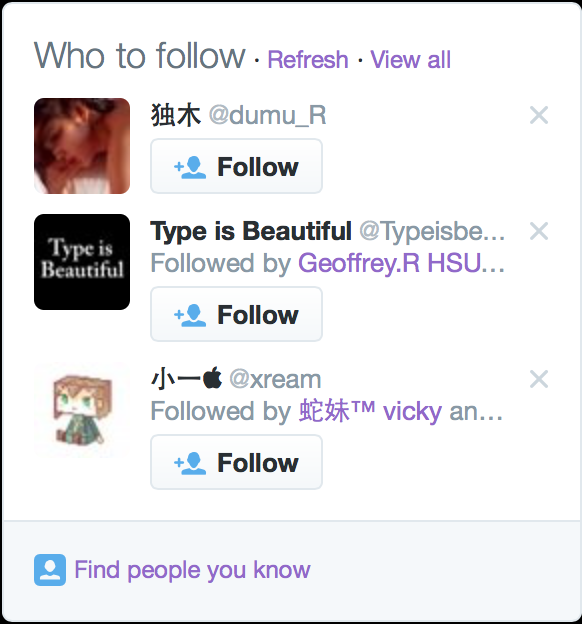
\includegraphics[width=\textwidth]{img/chap1/twitter_recommend.png}
\caption{flickr \label{Twitter推荐}}
\end{minipage}
\hfill
\begin{minipage}[t]{0.45\linewidth}
\centering

\includegraphics[width=\textwidth]{img/chap1/weibo_recommend.png}
\caption{instagram\label{weibo推荐}}
\end{minipage}

\end{figure}
虽然现在的方式各种各样,但无可否认的是至今不存在一种很好的方式提供给用户去拓展他们的社交圈子。

这就产生了本研究的一个最初的动机:

 \textbf{能否通过一种图片交流的方式提供图片类应用的用户去认识新朋友的渠道?}

而最近由于人脸识别技术的火热,市面上不断在涌现着与人脸识别关系密切的应用,比如face++与阿里巴巴在支付宝上联合推出的“刷脸”支付功能。

这些给予了笔者以灵感,笔者拟应用人脸的特征去提供一种独特的方式给用户去拓展他们的社交圈子,结合了传统的“夫妻脸“的概念,其中最基础的方式就是以人脸相似度去实现一个应用。之后通过实验的不断调整,加入其他特征去调整最后的好友推荐算法,得出最后的适合用户的匹配好友算法。
\section{方案概述}
􏰉􏴳􏰭􏴴􏴵􏴶􏴷􏰿􏴸􏴹􏴘􏰏􏲦􏲜􏱲􏴺􏰭􏴻􏲆􏴻􏴼􏰏􏱦􏴷􏱜􏰒􏴽􏳯􏴾􏴿􏵀􏱾􏱜本文提出基于人脸识别技术的图片社交平台,利用人脸识别的技术,不但能够提高人脸识别技术的通用性,并能提高用户对于社交应用的体验。根据不同的用户脸部特征,个人信息,本文对于基于用户特征值的匹配算法的可行性进行了系统的研究。基于已有的特征值,推荐给用户各项指标都符合其标准的好友,使得可以为用户提供一个良好的方式去扩展他们的社交圈。


因此对于图片社交应用的一种基于人脸识别方式的好友扩展方式的研究,基本的工作可以总结为如下:
\begin{enumerate}
\item 了解现有的社交应用给予用户的扩展好友的方式,调研相关的人脸识别的技术和算法,提出一种基于人脸特征的好友推荐匹配算法
\item 基于face++提供的api,完善在node.js平台上sdk的支持,并调研和准备应用的数据,存储到数据库中。
\item 基于angularJS+Ionic框架,开发出一款能够应用在三个移动手机平台上的应用。该应用不但能有效的解决用户好友来源的问题,并且可以在好友推荐中,为用户推荐符合用户的好友。同时,根据用户的反馈能够及时的调整对应的匹配算法。
\item 对于基于不同算法的好友推荐算法,进行实际的用户效果的测试,通过实验数据的比较取得一种较高满意度的推荐算法。实验结果表明本应用的好友推荐算法具有较高的实用价值和扩展性。
\end{enumerate}

% \section{研究的目的和意义}
\section{本文组织}
第一章包括背景和对研究的分析,及本文组织。第二章介绍论文相关技术和工作。第三章详细给出系统的算法和逻辑设计。第四章详细给出详细的系统的算法的。第五章进行总结和未来工作。
% 中文测试文字。
% \pkuthssffaq%


	% vim:ts=4:sw=4
% Copyright (c) 2014 Casper Ti. Vector
% Public domain.

\chapter{相关工作}


\section{人脸识别技术}
人脸识别\parencite{faceR}是一项热门的计算机技术研究领域,它属于生物特征识别技术,是对生物体(一般特指人)本身的生物特征来区分生物体个体。生物特征识别技术所研究的生物特征包括脸、指纹、手掌纹、虹膜、视网膜、声音(语音)、体形、个人习惯(例如敲击键盘的力度和频率、签字)等,相应的识别技术就有人脸识别、指纹识别、掌纹识别、虹膜识别、视网膜识别、语音识别(用语音识别可以进行身份识别,也可以进行语音内容的识别,只有前者属于生物特征识别技术)、体形识别、键盘敲击识别、签字识别等。
\subsection{Face++}
Face++是新一代云端视觉服务平台,提供一整套世界领先的人脸检测,人脸识别,面部分析的视觉技术服务。
Face++旨在提供简单易用,功能强大,平台通用的视觉服务,让广大的Web及移动开发者可以轻松使用最前沿的计算机视觉技术,从而搭建个性化的视觉应用。

Face++同时提供云端REST API以及本地API(涵盖Android, iOS, Linux, Windows, Mac OS),并且提供定制化及企业级视觉服务。通过Face++,可以轻松搭建云端身份认证,用户兴趣挖掘,移动体感交互,社交娱乐分享等多类型应用。
Face++提供了相应的http请求的接口,并提供了python,java,c++的API。

在本项目中,作者对于Face++对于nodejs的API进行了补全,能够很好的支持nodejs对于face++的接口应用,方便之后的nodejs开发者能够有效的利用该项技术。

\subsection{caffe}
Caffe( http://caffe.berkeleyvision.org/ )是一个清晰而高效的深度学习框架,其作者是博士毕业于UC Berkeley的贾扬清(http://daggerfs.com/ ),他目前在Google工作。Caffe是纯粹的C++/CUDA架构,支持命令行、Python和MATLAB接口,可以在CPU和GPU直接无缝切换。caffe在图像处理方面有着自己独特的效果。

\subsection{技术选用}
通过比较了这两项技术之后,由于Face++是专门做人脸识别的技术,他的各项评测也遥遥领先,所以在本文准备使用face++的API来实现应用。


\section{移动应用}
移动应用(Mobile application)安装和运行在移动设备上。它随着智能手机的推出,由于其移动性和娱乐性,在近年来达到了全新的巅峰。目前有三大主流的移动应用平台,分别为IOS,Android和Windows Phone。据三大平台统计,从2010年到2013年,移动应用的数目增加了100多万个。因此,移动应用是目前软件开发的一种最流行的模式,移动设备庞大的用户量和较小的开发经费也吸引了越来越多的自由开发者加入到了移动应用的开发者行列之中。
\subsection{angularJS}
angularJS是一款开源JavaScript函式库,由Google维护,用来协助单一页面应用程式运行的。它的目标是透过MVC模式(MVC)功能增强基于浏览器的应用,使开发和测试变得更加容易。
函式库读取包含附加自定义(标签属性)的HTML,遵从这些自定义属性中的指令,并将页面中的输入或输出与由JavaScript变量表示的模型绑定起来。这些JavaScript变量的值可以手工设置,或者从静态或动态JSON资源中获取。
AngularJS是建立在这样的信念上的:即声明式编程应该用于构建用户界面以及编写软件构建,而指令式编程非常适合来表示业务逻辑。 框架采用并扩展了传统HTML,通过双向的数据绑定来适应动态内容,双向的数据绑定允许模型和视图之间的自动同步。因此,AngularJS使得对DOM的操作不再重要并提升了可测试性。

设计目标:
\begin{enumerate}
\item 将应用逻辑与对DOM的操作解耦。提高代码的可测试性。
\item 将应用程序的测试看的跟应用程序的编写一样重要。代码的构成方式对测试的难度有巨大的影响。
\item 将应用程序的客户端与服务器端解耦。这允许客户端和服务器端的开发可以齐头并进,并且让双方的复用成为可能。
\end{enumerate}
指导开发者完成构建应用程序的整个历程:从用户界面的设计,到编写业务逻辑,再到测试。
\subsection{ionic}
Ionic\parencite{ionic}提供了一个免费且开源的移动优化HTML,CSS和JS组件库,来构建高交互性应用。基于Sass构建和AngularJS 优化,并形成了一个强大的 HTML5 应用程序开发框架,可以帮助使用 Web 技术,比如 HTML、CSS 和 Javascript 构建接近原生体验的移动应用程序。

Ionic 主要关注外观和体验,以及和你的应用程序的 UI 交互,特别适合用于基于 Hybird 模式的 HTML5 移动应用程序开发。且它是一个轻量的手机UI库,具有速度快,界面现代化、美观等特点。为了解决其他一些UI库在手机上运行缓慢的问题,它直接放弃了IOS6和Android4.1以下的版本支持,来获取更好的使用体验.


Ionic是现在GitHub上的最火的开源项目之一,具有超过16,000星及以上创建600000Ionic app。Ionic遵循视图控制模式,通俗的理解和 Cocoa 触摸框架相似。在视图控制模式中,我们将界面的不同部分分为子视图或包含其他视图的子视图控制器。然后视图控制器“驱动”内部视图来提供交互和UI功能。一个很好的例子就是标签栏(Tab Bar)视图控制器处理点击标签栏在一系列可视化面板间切换。
\subsection{技术选用}
相较于原生的Android,IOS,Windows Phone应用,于angularJS+ionic的框架实现的应用在三大平台都能够使用,存在了很强大的适用性,能够针对更多的用户,并且针对于现有先进的移动设备有了一个较好的实用性。
\section{数据库调研}
为了收集可用的用户信息,建立一个叫完整的图片数据库,我们需要调研一个基础的能够供我们对于用户的实验数据库。
\subsection{mongodb}
Mongo DB 是目前在IT行业非常流行的一种非关系型数据库(NoSql),其灵活的数据存储方式备受当前IT从业人员的青睐。Mongo DB很好的实现了面向对象的思想(OO思想),在Mongo DB中 每一条记录都是一个Document对象。

Mongo DB最大的优势在于所有的数据持久操作都无需开发人员手动编写SQL语句,直接调用方法就可以轻松的实现CRUD操作。
MongoDB的文档模型自由灵活,可以让你在开发过程中畅顺无比。对于大数据量、高并发、弱事务的互联网应用,MongoDB可以应对自如。MongoDB内置的水平扩展机制提供了从百万到十亿级别的数据量处理能力,完全可以满足Web2.0和移动互联网的数据存储需求,其开箱即用的特性也大大降低了中小型网站的运维成本。

\subsection{数据来源}
根据本文所要实现的应用的特性,是基于人脸的社交应用,而无疑最符合这个性质的社交应用就是婚恋市场的社交应用。
而也只有婚恋的用户才会在大概率上将他们的真实人物照片提交到应用上,为了模拟这个应用的特性,本文实验的数据库的来源也需要从类似的网站上抓取,排除掉国外的婚恋网站,作为国内的比较流行的婚恋网站有,百合网,珍爱网,世纪佳缘。


通过比较这几个网站的数据,发现百合网的会员资料的开放程度不及世纪佳缘,珍爱网。而世纪佳缘的用户活跃度和注册数远远优于珍爱网。所以本文拟用世纪佳缘的数据作为本文应用的数据库来源。

\section{爬虫}
\subsection*{Beatifulsoup}
Beautiful Soup提供一些简单的、python式的函数用来处理导航、搜索、修改分析树等功能。它是一个工具箱,通过解析文档为用户提供需要抓取的数据,因为简单,所以不需要多少代码就可以写出一个完整的应用程序。Beautiful Soup自动将输入文档转换为Unicode编码,输出文档转换为utf-8编码。你不需要考虑编码方式,除非文档没有指定一个编码方式,这时,Beautiful Soup就不能自动识别编码方式了。然后,你仅仅需要说明一下原始编码方式就可以了。Beautiful Soup已成为和lxml、html6lib一样出色的python解释器,为用户灵活地提供不同的解析策略或强劲的速度。


% % 中文测试文字。
% \pkuthssffaq


	% vim:ts=4:sw=4
% Copyright (c) 2014 Casper Ti. Vector
% Public domain.

\chapter{系统设计}

\section{匹配算法设计}
对于匹配算法的设计,主要的思想是探究出一种基于用户特征信息来推荐与用户志趣相投的人,所以其中必须要考虑到是现实用户对匹算算法实际效果的满意程度。之后对于不同的意见,对于匹配算法再进行不断对应的调整,从而得到一个相对最优的算法。故此,本文准备采取不同的匹配算法来实验,选取出实验效果最好的来当作最终实施在应用上的算法。同时,该算法可以根据用户的反馈来调整用户的信息的适应性,从而实现程序的自动调节。
\subsection{基于人脸相似度的算法设计}
设变量。。以f当作人脸相似度
 \begin{equation}
   C = \mathop{\argmax}_{c}{\sum_t{w^t_c}}%find how to write down the scripts.
 \end{equation}

\subsection{基于用户信息的算法设计}
根据用户提供的信息,将此当作一个变量添加到匹配算法中,将用户信息提供的信息i设为xi,而对应不同的信息i应该具有不同的匹配算法fi,举个例子,比如年龄信息的可用正态分布的函数对于推荐用户年龄的进行一个匹配,即fi(xi)=正态分布函数。

由此我们可以推导出我们新的

但由于用户的兴趣问题,我们针对于用户的猜测可能导致负相关,因此这里的变量越少越好。
\subsection{基于机器学习的算法设计}

\section{应用端设计}

根据社交应用的性质,关于应用端的逻辑应该能够提供给用户能够查看,交流,以及使用最主要的匹配功能,所以本文implement的应用端的逻辑如下图所示
[用苹果的view画一个图]
其中第一个View是主界面来展示用户的post信息,点入具体的一个card,对应着具体的用户的post信息。

\section{face++ SDK for node.js}
由于Face++并没有提供对应的SDK给node.js,所以本研究需要为face++的http请求的api实现一个SDK给node.js。Face++的API如下图


\section{服务器设计}
[用omnigraffle画一个思维导图]


\section{数据库设计}

[用er图]
[用mysql画的一个图]

% 中文测试文字。



	% vim:ts=4:sw=4
% Copyright (c) 2014 Casper Ti. Vector
% Public domain.

\chapter{系统实现}
\section{爬虫模块}
基于在本文第二部分中的数据来源和爬虫的分析,采用beautifulSoup技术来进行爬取数据。
% \subsection{爬取基本数据}
\begin{figure}[h]
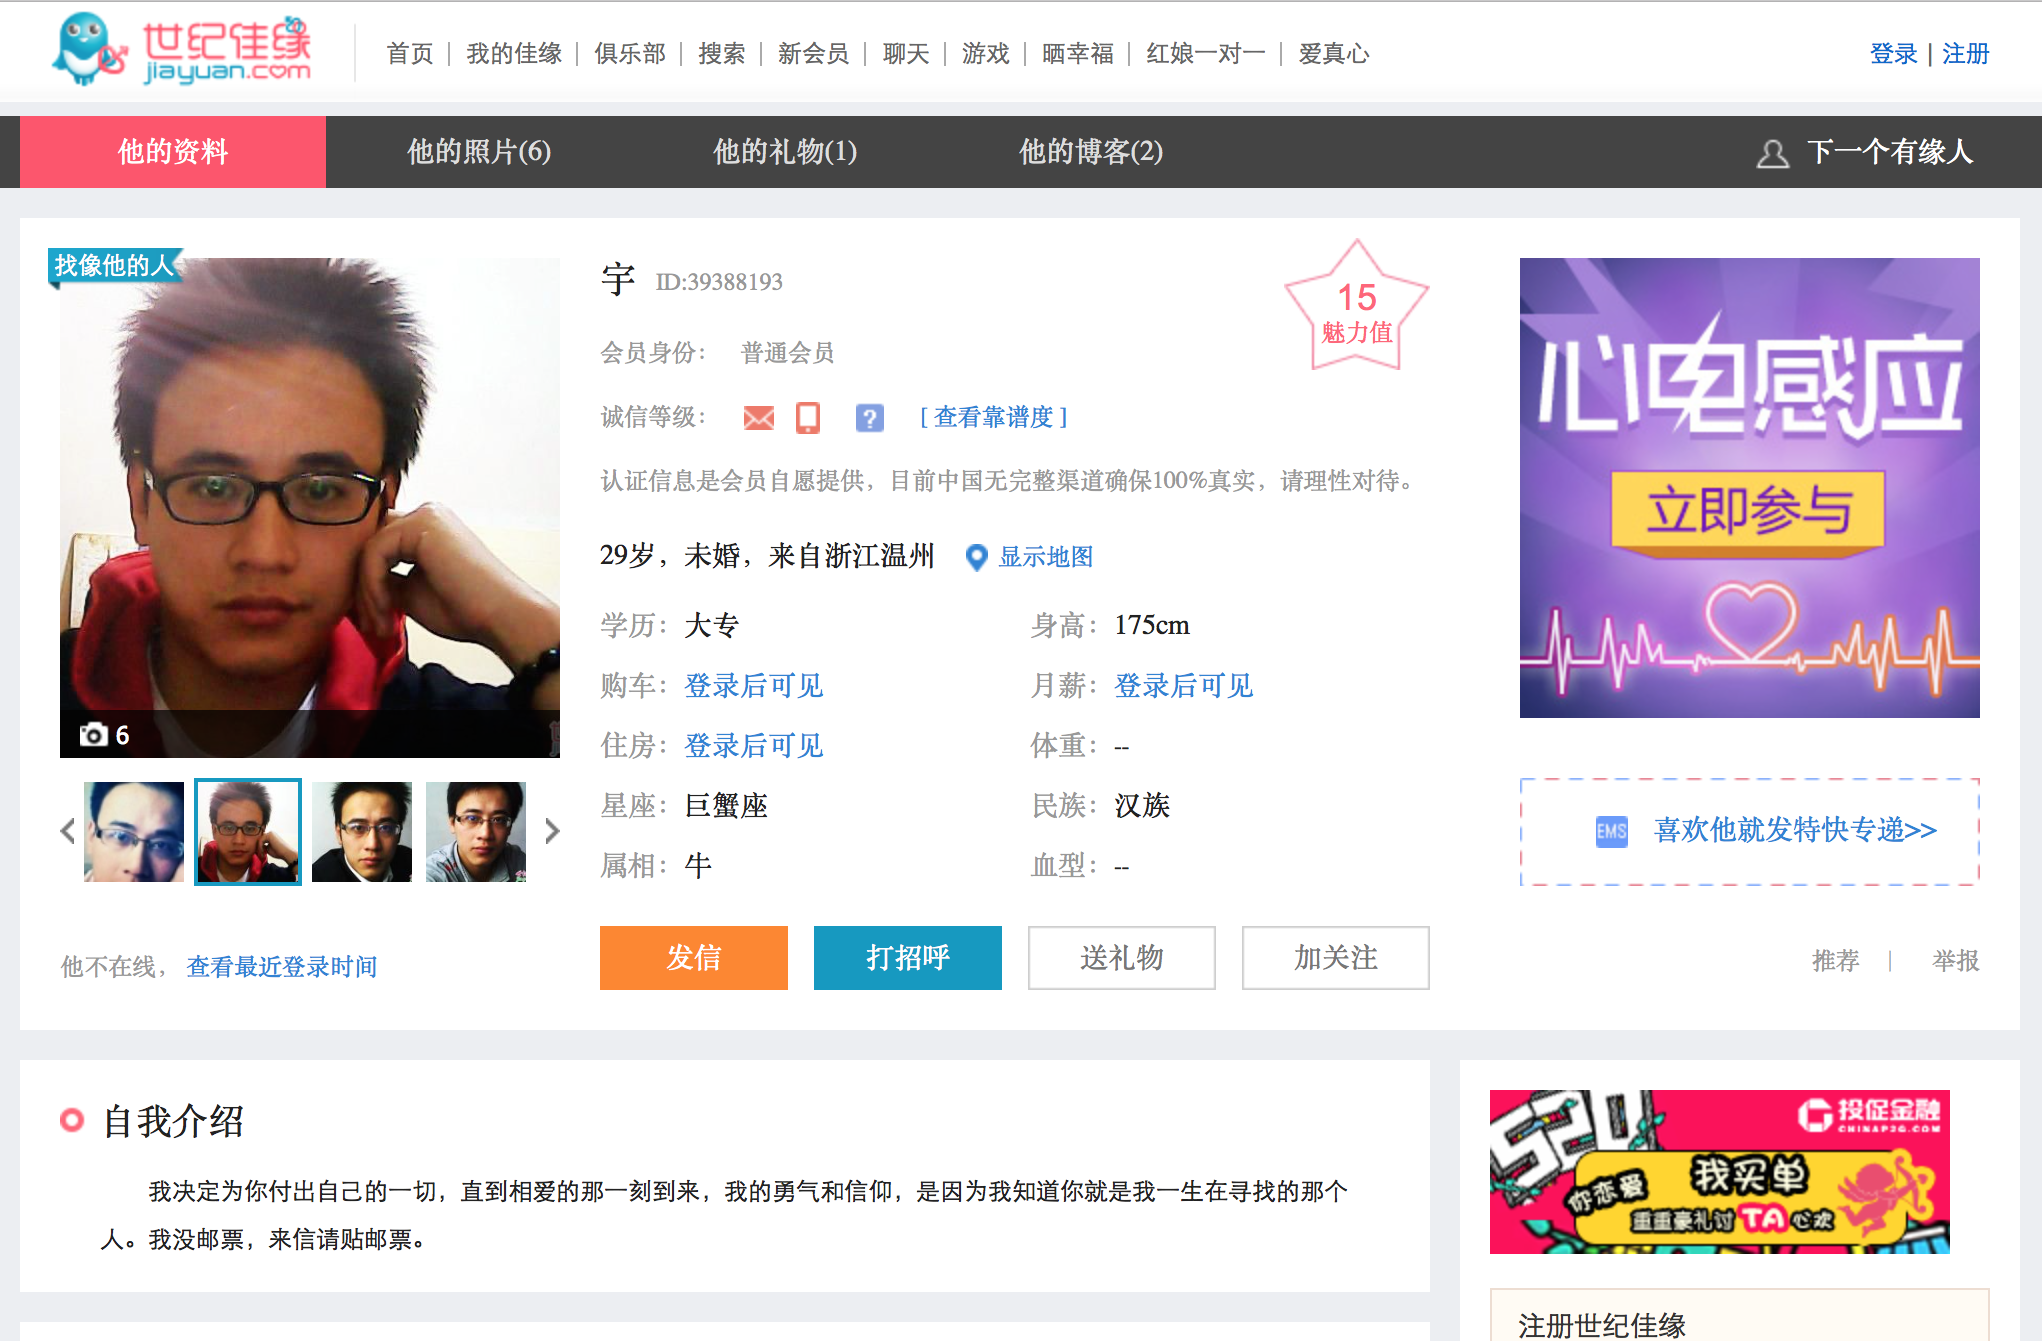
\includegraphics[width=\textwidth]{img/chap4/jiayuan1.png}
\caption{世纪佳缘用户信息页面\label{Face++API}}
\end{figure}
% \begin{figure}[h]
% 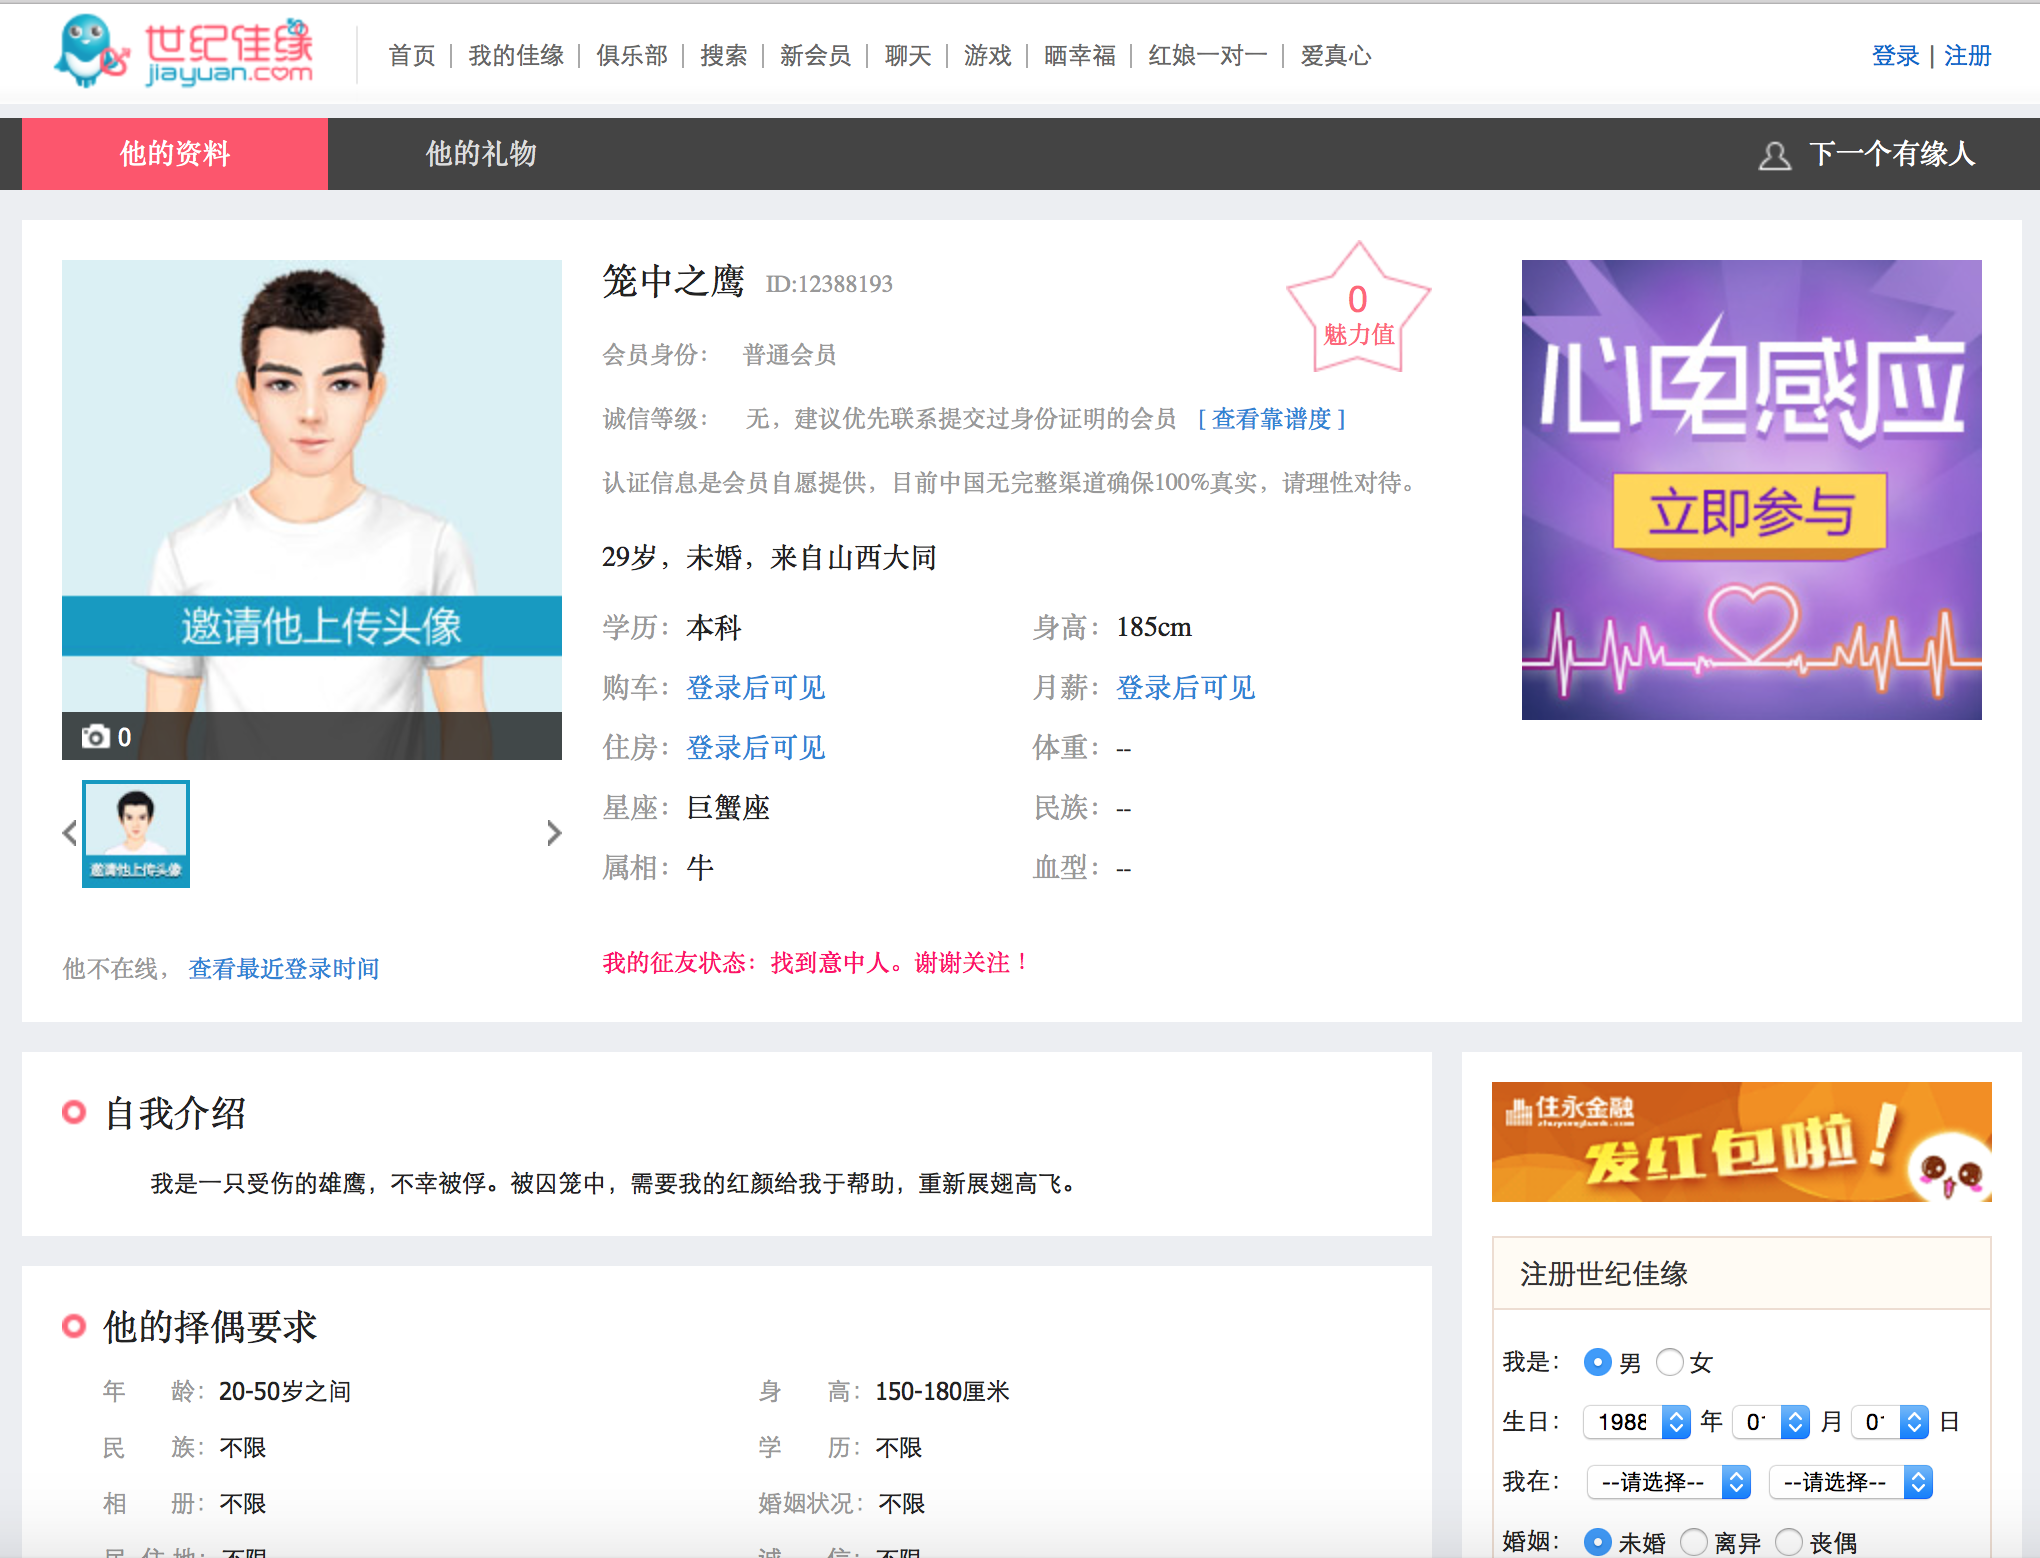
\includegraphics[width=\textwidth]{img/chap4/jiayuan2.png}
% \caption{世纪佳缘需权限信息页面\label{Face++API}}
% \end{figure}

通过前期充分对于世纪佳缘网站的调研,对于用户信息的分析,针对用户数据的发掘,本文找到了一个基于用户id以及对应用户数据联系的网页,从图4.1可以看出,此网页url可以连接到用户id具体的用户信息,从而我们可以针对指定的用户进行必要的信息的爬取。

但在实际操作中,一些用户的图片和信息设置为成权限可见之外,我们因此在程序中需要排除掉此类非法数据。除此之外其他的数据对于爬虫都是友好的,并且在一定程度上提供了丰富的用户信息,以便于我们进行匹配算法的优化。

最后我们的爬虫脚本对于抓取到的数据信息,存储到到本文的用户人脸数据库之中。

我们的爬虫的算法可以抽象成如下的伪代码。

\begin{codebox}
\Procname{$\proc{Crawler}$}
\li \For $j \gets $ \To the Amount of extrace \label{li:for}
\li     \Do \label{li:for-begin}
\li 	$URL \gets$ crawler url 
\li 	$Data \gets$ Raw data from $URL$
\li 	\For $k \gets$ Rule of Elements to form Data \label{li:for}
\li     	\Do \label{li:for-begin}
\li 		$info /gets$ information from $Data$ regulated by $k$
\li      	Insert $Info$ into the sorted sequence $Request$.
\label{li:for-end}
                \End
\li         Connect database submit $Request$ to database       \label{li:for-end}
        \End
\end{codebox}

该算法大致的思路如下:
\begin{itemize}
\item 确定爬取URL的个数
\item 循环,对于每个URL,从网页端爬取原始信息。
\item 对于每一个需求的信息的特征,进行不同的规则选取。
\item 对于特定的规则,在原始信息中提取特征信息
\item 将特征信息存入临时的表中
\item 连接数据库,将临时数据提交至数据库
\end{itemize}
% [伪代码1]
% \subsection{导入数据库}

% [伪代码2]

\section{应用端模块}
该应用的实现由三步组成:状态查询,信息源添加,和匹配反馈。


\subsection{状态查询及展示}
为了满足用户自己查询感兴趣好友的需求,应用需要提供用户在使⽤应⽤程序查看他人已经存在的Post信息。并为了便携性和可用性,需完成进行对于用户Post信息的一个预览,以及对于具体Post信息的查询。

从而可以满足用户的需求,去查看其他用户Post具体的信息,并可以支持用户随时对于需要的信息的刷新,以及链接用户更进一步的个人主页的途径。
\begin{figure}[h] 
\begin{minipage}[t]{0.3\linewidth}
\centering
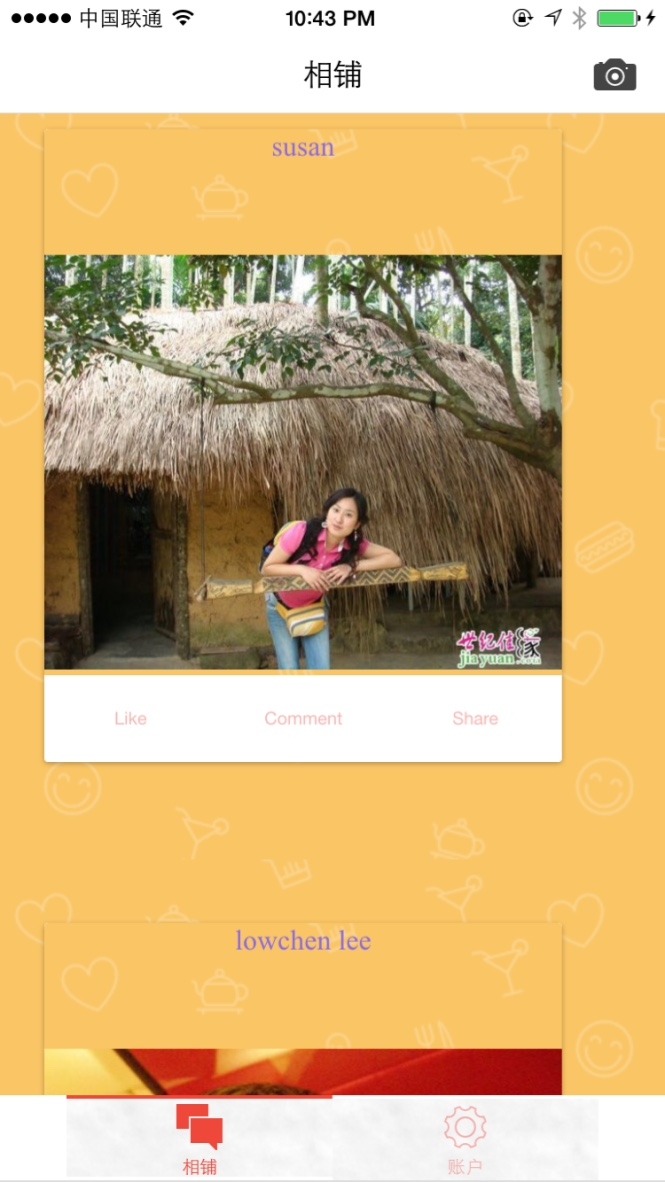
\includegraphics[width=\textwidth]{img/chap4/info1.jpg}
\caption{主界面\label{flickr}}
\end{minipage}
\hfill
\begin{minipage}[t]{0.3\linewidth}
\centering
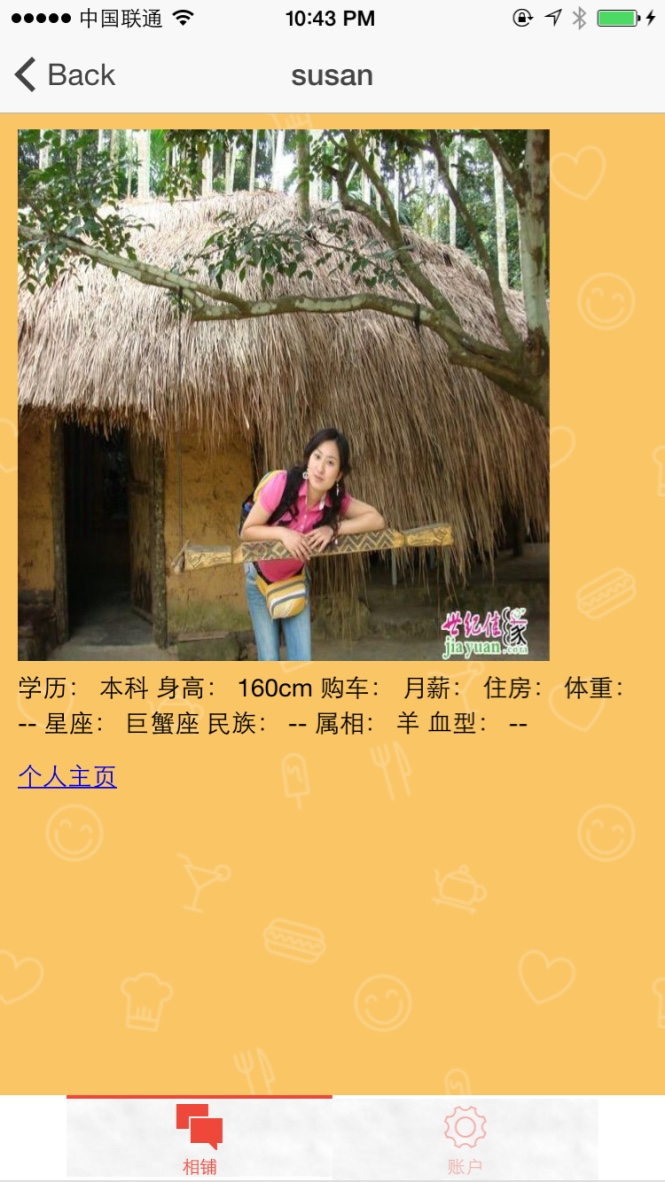
\includegraphics[width=\textwidth]{img/chap4/info2.jpg}
\caption{详细信息\label{instagram}}
\end{minipage}
\hfill
\begin{minipage}[t]{0.3\linewidth}
\centering
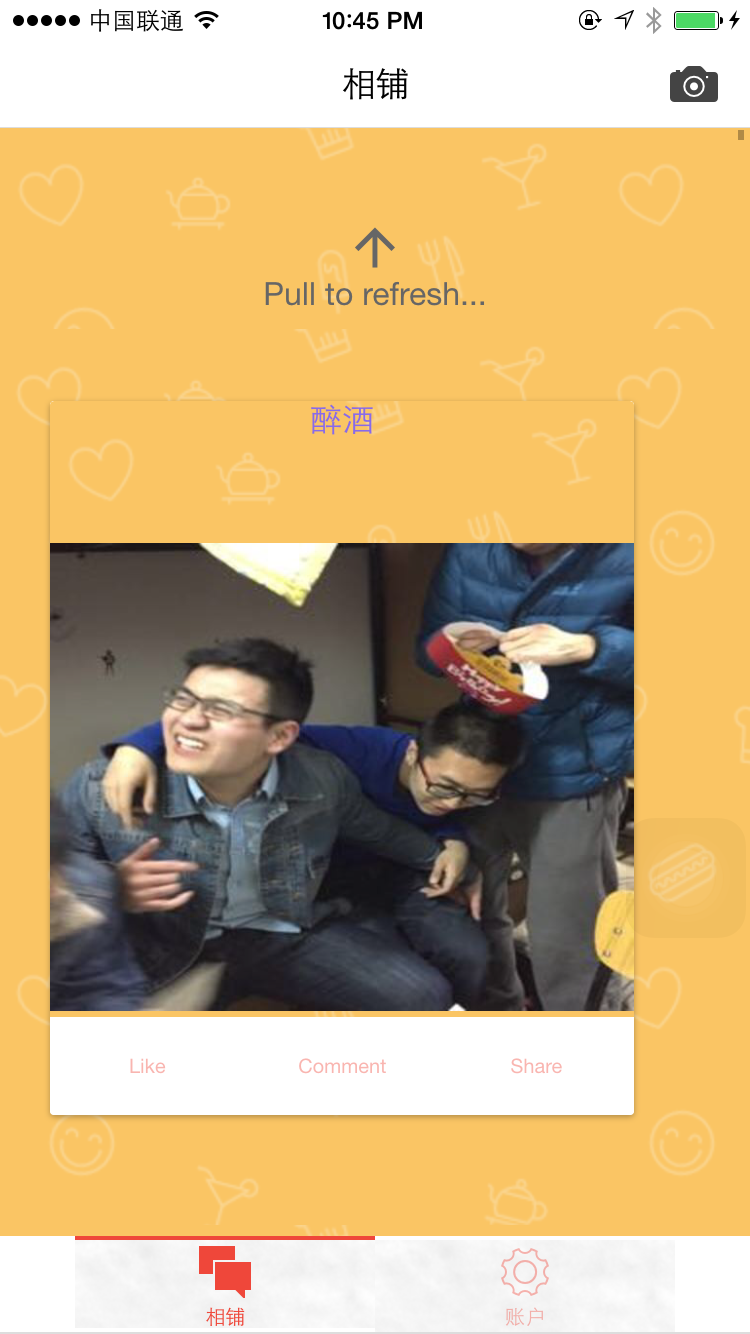
\includegraphics[width=\textwidth]{img/chap4/info3.PNG}
\caption{刷新\label{snapchat}}
\end{minipage}
\hfill
\end{figure}

进入应用,我们首先进入了主界面(图4.2所示),在这里我们可以看到用户Post的缩略图,既省略了用户的Post详细信息,可以达到快速浏览的目点,又为用户提供了一个可以找到自己兴趣点的信息。

如果对一个用户感兴趣,点击即可转到详细信息界面(图4.3所示),显示了用户Post的详细信息。

为了及时更新Post,主界面补充了刷新功能(图4.4所示),可以对主界面的Post进行刷新。

\subsection{信息源添加}
用户关于自己信息的发布通常希望其发布的信息具有多种多样的形式,考虑到移动设备较难编辑和显⽰富⽂本信息,应⽤用程序被实现为能够编辑、存储和显示具有多种类型的字段,包括个人姓名、个人介绍、URL和提交的匹配图片

并且基于用户照片来源的不同,分为从用户的图片库中采集和即时照相两种不同图片来源方式。并在此基础上实现了图片预览的功能。
\begin{figure}[h] 
\begin{minipage}[t]{0.3\linewidth}
\centering
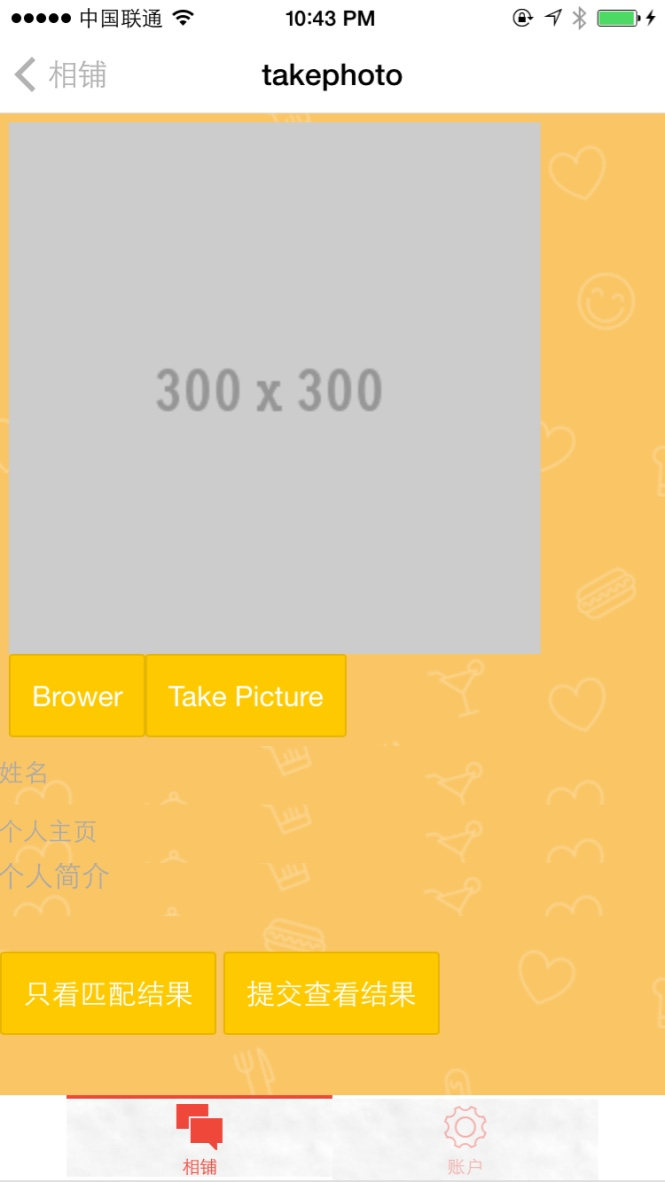
\includegraphics[width=\textwidth]{img/chap4/take1.jpg}
\caption{提交界面\label{flickr}}
\end{minipage}
\hfill
\begin{minipage}[t]{0.3\linewidth}
\centering
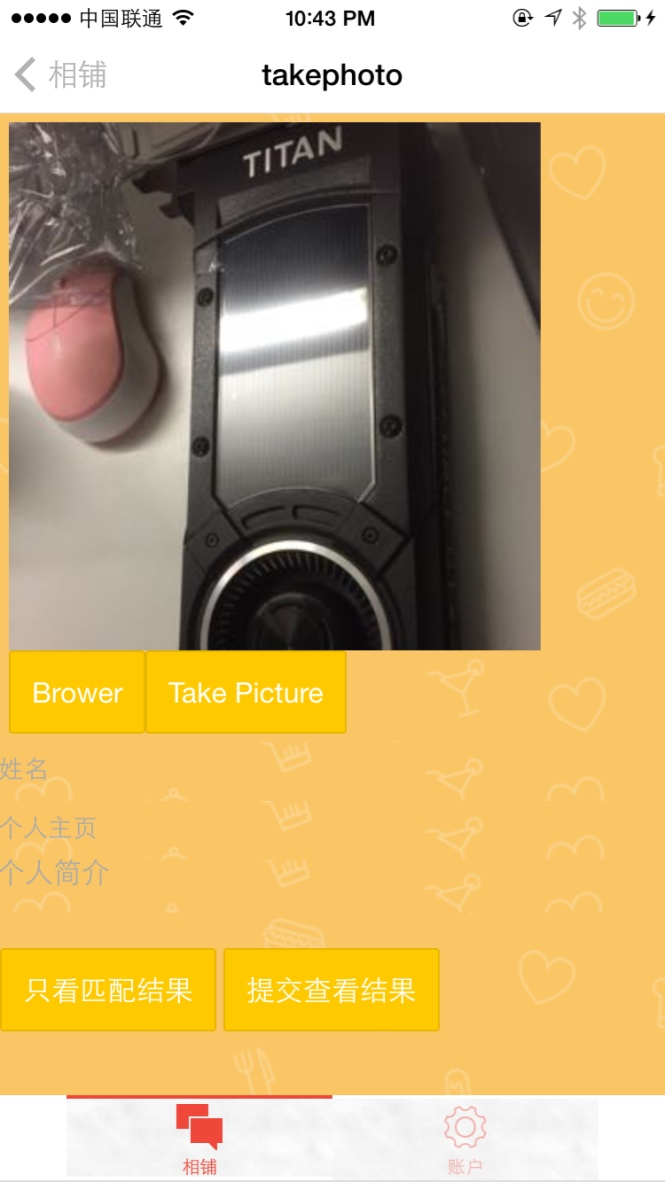
\includegraphics[width=\textwidth]{img/chap4/take2.jpg}
\caption{预览提交的图片\label{instagram}}
\end{minipage}
\hfill
\begin{minipage}[t]{0.3\linewidth}
\centering
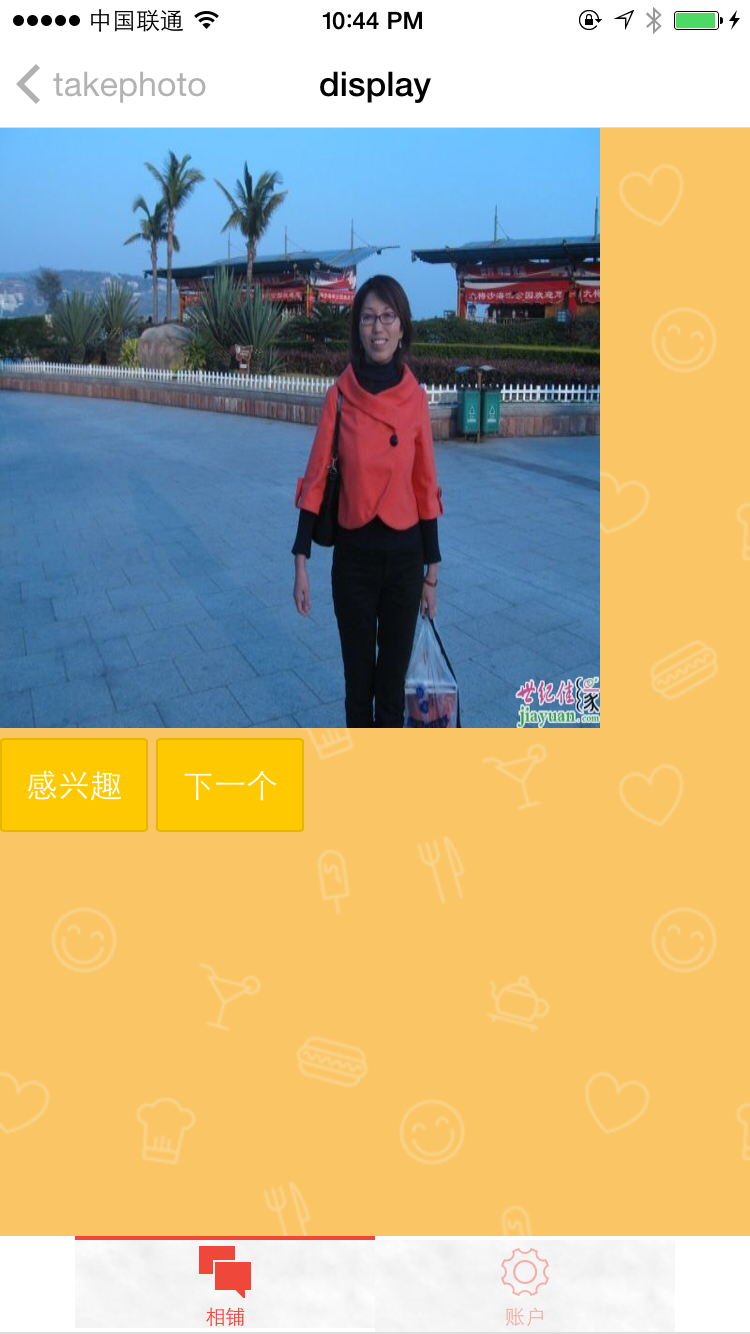
\includegraphics[width=\textwidth]{img/chap4/display.PNG}
\caption{展示界面\label{instagram}}
\end{minipage}



\end{figure}
图4.5和4.6展示了这两项功能,提供用户描述自己Post信息的通道,并使得用户能够通过不同的方式提供自己的人脸图片,并预览自己提交的图片。
\subsection{匹配信息展⽰}
由于服务端有客户端提交的图片以及文本信息直接调用对应匹配算法的接口,因此,应用端在用户在提交了自己的信息之后可以直接调用了此接口,服务端便具有了足够的信息以匹配出对应的好友。

在服务端返回给客户端匹配出的结果后,客户端将详细信息显⽰在⽤用户界⾯上(图4.7所示)。这里具有具有多条匹配结果,客户端将按照匹配程度顺序将结果显⽰。当用户对该用户感兴趣时即点击“感兴趣”按钮进入查询详细信息。





	% vim:ts=4:sw=4
% Copyright (c) 2014 Casper Ti. Vector
% Public domain.

\chapter{总结和展望}
\section{系统测试}
为了分析和评估本论文提出的基于人脸识别的匹配算法的有效性和可用性,我们使用了该算法编写的基于婚恋数据的匹配好友的应用进行了实验测试。本实验主要真了基于不同算法的匹配系统进行了分析评估。
\subsection{数据库用户分析}
根据数据库的特性和年龄地区分布
[用户年龄分布图]
[用户地区分布图]
\subsection{实验结果}
本实验

由于在设计的每⼀一个阶段对系统的性能和可扩展性都提出了要求,最后实现的 系统具有良好的性能和可扩展性。虽然随着信息源的增多,算法耗时会变长,但接 近线性的时间复杂度使得耗时的增长处于可控的范围内,并且可以通过设置每个服 务器的服务范围使其对于每次请求的计算量维持在⼀一定的⽔水平。随着⽤用户的增多, 由于服务器可以横向扩展,只需增加服务器实例的数量便可应对更多的请求、保持一定的响应速度。

% \section{匹配算法实验}
% \subsection{根据人脸相似度的匹配}
% \subsection{根据具体人脸特征的匹配}
% \subsection{根据具体信息的匹配算法}
% \subsection{机器学习算法}


\section{展望}

\subsection{基于用户特点喜好的更进一步的匹配算法}

	% 结论。
	% vim:ts=4:sw=4
% Copyright (c) 2014 Casper Ti. Vector
% Public domain.

\specialchap{本文总结}
% 中文测试文字。
% \pkuthssffaq

本文提出了一种新型的图片社交平台,通过人脸识别技术为主导的好友推荐匹配来有效的扩展用户的社交圈以及提升用户活跃的程度。在本应用中用户可以通过他们的信息特征来寻找与他们兴趣相符的好友。

本文实现了基于angularJS+ionic的客户端应用程序,以及以世纪佳缘为数据源导入的数据库,以face++API实现的nodejs的SDK,已经对应的服务器程序。目前的实验表明本文的匹配算法具有良好的用户体验,能够有效的为用户提供适合用户特征的好友,具有良好的可扩展性和实用性。

实验数据毕竟具有一定的随机性,且得到的数据较为主管,因此在之后为了更好的去探索人脸识别技术图片社交平台上的应用,需要在之后我们考虑更广泛的实验,并且将此应用发布并推广出去去获得更多的用户的反馈进一步来精确原算法的阈值,获得更多用户的特征数据来提升算法。

而在图片识别等技术的飞速发展上,应用能够更多的通过图片来收集用户的信息,将用户的日常信息不断分类,从而更为精确的为用户匹配好友。我们可以期待图片社交应用更远大的未来。





	% 正文中的附录部分。
	\appendix
	% 排版参考文献列表。
	\printbibliography[
		% 使“参考文献”出现在目录中;如果同时要使参考文献列表参与章节编号,
		% 可将“bibintoc”改为“bibnumbered”。
		heading = bibintoc,
		% 单独设定排序方案。此设定会局部覆盖之前的全局设置。
		% 注:只有同时使用 2.x 或之后版本的 biblatex 和相应兼容版本的 biber,
		% 才能对每个 \printbibliography 命令采用不同的排序方案,
		% 否则只能在载入 biblatex 宏包时就(全局)指定排序方案。
		% 在这样的情况下,请去掉所有的 sorting 选项,否则可能出错。
		sorting = ecnty
	]
	% 各附录。
	% vim:ts=4:sw=4
% Copyright (c) 2014 Casper Ti. Vector
% Public domain.

\chapter{附件}
% 中文测试文字。
\pkuthssffaq



	% 以下为正文之后的部分,默认不进行章节编号。
	\backmatter
	% 致谢。
	% vim:ts=4:sw=4
% Copyright (c) 2014 Casper Ti. Vector
% Public domain.

\chapter{致谢}
% 中文测试文字。
% \pkuthssffaq
感谢我的母校北京大学,燕园浓厚的学术氛围,培养了一代代社会精英,
祖国栋梁。与良师益友交游,谈笑有鸿儒,往来无白丁,这里的寸寸土地,都
充满了智慧与知识。
  感谢所有教授过我各类课程的老师。他们丰富的学术积淀和睿智博学的个
人风采都让我崇敬仰慕。
  感谢北京大学网络与信息系统研究所移动网络组为我提供的良好的实验环
境。
感谢边凯归老师和严伟老师,他们在我的工具实现,实验完成和论文写作 方面给予了我充分的指导和鼓励。在进入移动网络组一年的时间里,我切身感 受到边老师与严老师亲切的师长风采与迷人的学术魅力,每一次和老师的交流, 都能得到许多启迪和灵感,这都是我人生中最宝贵的财富。
  感谢实验室和与我同级的同学还有朋友们:毛景树,薛易清,等等等等,他们在我的论文写作中,为我提供了充分的帮助,使我克服了许多
困难,少走了许多弯路。还有很多参与了我毕设实验的亲人朋友还有同学们,
正是有了他们对我的帮助,使我得以顺利完成本论文。
  感谢我的父母,无论寒暑春秋都给我最无私的支持和鼓励。感谢所有关心
我的亲人和朋友以及所有给与我帮助的人,我的每一份收获都离不开你们。



	% 此后不排版页眉或页脚。
	% \cleardoublepage
	\pagestyle{empty}

	% 原创性声明和使用授权说明。
	% vim:ts=4:sw=4
%
% Copyright (c) 2008-2009 solvethis
% Copyright (c) 2010-2015 Casper Ti. Vector
% All rights reserved.
%
% Redistribution and use in source and binary forms, with or without
% modification, are permitted provided that the following conditions are
% met:
%
% * Redistributions of source code must retain the above copyright notice,
%   this list of conditions and the following disclaimer.
% * Redistributions in binary form must reproduce the above copyright
%   notice, this list of conditions and the following disclaimer in the
%   documentation and/or other materials provided with the distribution.
% * Neither the name of Peking University nor the names of its contributors
%   may be used to endorse or promote products derived from this software
%   without specific prior written permission.
%
% THIS SOFTWARE IS PROVIDED BY THE COPYRIGHT HOLDERS AND CONTRIBUTORS "AS
% IS" AND ANY EXPRESS OR IMPLIED WARRANTIES, INCLUDING, BUT NOT LIMITED TO,
% THE IMPLIED WARRANTIES OF MERCHANTABILITY AND FITNESS FOR A PARTICULAR
% PURPOSE ARE DISCLAIMED. IN NO EVENT SHALL THE COPYRIGHT HOLDER OR
% CONTRIBUTORS BE LIABLE FOR ANY DIRECT, INDIRECT, INCIDENTAL, SPECIAL,
% EXEMPLARY, OR CONSEQUENTIAL DAMAGES (INCLUDING, BUT NOT LIMITED TO,
% PROCUREMENT OF SUBSTITUTE GOODS OR SERVICES; LOSS OF USE, DATA, OR
% PROFITS; OR BUSINESS INTERRUPTION) HOWEVER CAUSED AND ON ANY THEORY OF
% LIABILITY, WHETHER IN CONTRACT, STRICT LIABILITY, OR TORT (INCLUDING
% NEGLIGENCE OR OTHERWISE) ARISING IN ANY WAY OUT OF THE USE OF THIS
% SOFTWARE, EVEN IF ADVISED OF THE POSSIBILITY OF SUCH DAMAGE.

% 原创性声明和使用授权说明页不需要装订到论文中,故不显示页码。
\cleardoublepage\thispagestyle{empty}
{
	\vspace*{\fill}\linespread{1.5}\selectfont
	\centerline{\bfseries\zihao{-2}北京大学学位论文原创性声明和使用授权说明}

	\vskip 4em
	\centerline{\bfseries\zihao{-3}原创性声明}
	\vskip 1em

	本人郑重声明:
	所呈交的学位论文,是本人在导师的指导下,独立进行研究工作所取得的成果。
	除文中已经注明引用的内容外,
	本论文不含任何其他个人或集体已经发表或撰写过的作品或成果。
	对本文的研究做出重要贡献的个人和集体,均已在文中以明确方式标明。
	本声明的法律结果由本人承担。
	\vskip 1em
	\rightline
	{%
		论文作者签名:\hspace{5em}%
		日期:\hspace{2em}年\hspace{2em}月\hspace{2em}日%
	}

	\vskip 4em
	\centerline{\bfseries\zihao{-3}学位论文使用授权说明}
	\centerline{\zihao{5}(必须装订在提交学校图书馆的印刷本)}
	\vskip 1em

	本人完全了解北京大学关于收集、保存、使用学位论文的规定,即:
	\begin{itemize}
		\item 按照学校要求提交学位论文的印刷本和电子版本;
		\item 学校有权保存学位论文的印刷本和电子版,
			并提供目录检索与阅览服务,在校园网上提供服务;
		\item 学校可以采用影印、缩印、数字化或其它复制手段保存论文;
		\item 因某种特殊原因需要延迟发布学位论文电子版,
			授权学校在 $\square$\nobreakspace{}一年 / %
			$\square$\nobreakspace{}两年 / %
			$\square$\nobreakspace{}三年以后在校园网上全文发布。
	\end{itemize}
	\centerline{(保密论文在解密后遵守此规定)}
	\vskip 1em
	\rightline
	{%
		论文作者签名:\hspace{5em}导师签名:\hspace{5em}%
		日期:\hspace{2em}年\hspace{2em}月\hspace{2em}日%
	}

	% 若需排版二维码,请将二维码图片重命名为“barcode”,
	% 转为合适的图片格式,并放在当前目录下,然后去掉下面 2 行的注释。
	%\vskip 4em \noindent
	%\includegraphics[height = 5em]{barcode}

	\vspace*{\fill}\par
}


\end{document}

